% Evans 6.5: English printed p.333 / PDF p.350; Chinese printed p.236 / PDF p.254.
\Needspace{65mm}
\section{Eigenvalues and Eigenfunctions}
\label{sec:6-5}
Assume in this section that $U$ is bounded, connected and has smooth
boundary, and that all coefficients are smooth on $\overline U$.
This keeps the spectral arguments separate from technical boundary
regularity issues. Eigenfunctions have zero Dirichlet trace.

\subsection{Symmetric operators (Evans \S6.5.1, Theorem 1)}
First let $Lu=-\partial_j(a^{ij}u_i)$ with $A$ symmetric uniformly elliptic.
Then $B[u,v]=\int A Du\cdot Dv$ is a symmetric positive form.
\begin{theorem}\label{thm:6-symmetric-spectrum}
There are real eigenvalues, repeated according to multiplicity,
\[
 0<\lambda_1\leq\lambda_2\leq\cdots,\qquad\lambda_j\longrightarrow\infty,
\]
and a complete orthonormal basis $(w_j)$ of $L^2(U)$ such that
$Lw_j=\lambda_jw_j$. Each eigenspace is finite dimensional, and
$w_j\in C^\infty(\overline U)$.
\end{theorem}
\begin{expandedproof}
Let $S=L^{-1}:L^2\to L^2$. Lax--Milgram, Poincar\'e and Rellich show
that $S$ is bounded and compact. If $u=Sf$ and $v=Sg$, then
\[
 (Sf,g)=B[u,v]=(f,Sg),\qquad
 (Sf,f)=B[u,u]>0\quad(f\ne0).
\]
Thus $S$ is self-adjoint, positive definite, and injective.

For completeness we give the compact spectral argument.
Let $\mu_1=\sup_{\|f\|_2=1}(Sf,f)>0$.
For a maximizing sequence $f_k$, pass to a weakly convergent subsequence
$f_k\rightharpoonup f$ with $\|f\|_2\leq1$.
Compactness gives $Sf_k\to Sf$, so $(Sf,f)=\mu_1$.
If $\|f\|_2<1$, scaling $f$ to norm one increases this value, a
contradiction. First variation on the unit sphere gives $Sf=\mu_1 f$.

Its orthogonal complement is invariant under $S$, by self-adjointness.
Repeat the argument there, recording multiplicities, to obtain
$\mu_1\geq\mu_2\geq\cdots>0$ and orthonormal eigenvectors $w_j$.
There are infinitely many, since an injective operator on infinite
dimensional $L^2(U)$ cannot have finite-dimensional range.
Compactness forces $\mu_j\to0$: otherwise $(Sw_j)$ has pairwise distances
bounded below.
If the closed span of the $w_j$ had a nonzero orthogonal complement,
the restriction of $S$ to that complement would still be compact and
positive definite and hence would have a positive maximal eigenvalue.
That value would be at most every $\mu_j$, contradicting $\mu_j\to0$.
This proves completeness. Set $\lambda_j=\mu_j^{-1}$.
Finite multiplicity follows from compactness, and regularity bootstrapping
applied to $Lw_j=\lambda_jw_j$ gives smoothness.
\end{expandedproof}
\Needspace{45mm}
\PDEAnnotation{先研究紧的逆算子}{$L$ 在 $L^2$ 上是无界算子，不宜直接套紧算子的谱定理。其逆先提升到 $H^1_0$，再由紧嵌入回到 $L^2$；逆的特征值趋零，对应 $L$ 的特征值趋无穷。}

\Needspace{35mm}
\subsection{Rayleigh quotient and positivity (Evans \S6.5.1, Theorem 2)}

\Needspace{45mm}
\PDEAnnotation{能量空间中的归一化不同}{$w_j$ 在 $L^2$ 中长度为一，但能量长度是 $\sqrt{\lambda_j}$。因此能量空间的正交归一基是 $w_j/\sqrt{\lambda_j}$，这决定了能量展开中的权重。}
\begin{theorem}\label{thm:6-rayleigh}
The first eigenvalue satisfies
\[
 \lambda_1=\min_{\substack{u\in H^1_0(U)\\\|u\|_2=1}}B[u,u].
\]
A minimizer solves $Lu=\lambda_1u$. There is a strictly positive first
eigenfunction in $U$, and $\lambda_1$ is simple.
Every eigenfunction for a larger eigenvalue changes sign.
\end{theorem}
\begin{expandedproof}
The energy inner product is $B$, equivalent to the $H^1_0$ norm.
The functions $w_j/\sqrt{\lambda_j}$ are orthonormal for this inner product,
since $B[w_i,w_j]=\lambda_i(w_i,w_j)$.
They are complete in the energy space: if $B[u,w_j]=0$ for all $j$,
then $(u,w_j)=0$ for all $j$, hence $u=0$ by the $L^2$ basis.
Hilbert-space Parseval therefore gives
\begin{equation}\label{eq:6-energy-spectrum}
 B[u,u]=\sum_j\lambda_j|(u,w_j)|^2,\qquad
 \|u\|_2^2=\sum_j|(u,w_j)|^2 .
\end{equation}
The Rayleigh minimum follows, with equality at $w_1$.
Alternatively, the direct method gives a minimizer: bounded energy
gives weak $H^1_0$ convergence, Rellich preserves the $L^2$ normalization,
and weak lower semicontinuity preserves minimality.

Differentiating the quotient
$B[u+tv,u+tv]/\|u+tv\|_2^2$ at $t=0$ yields
$B[u,v]=\lambda_1(u,v)$ for every $v$.
If $u$ is a minimizer, $|u|\in H^1_0$ has the same norm and energy
by the Sobolev chain rule, so it is also a minimizer and hence smooth.
It satisfies $L|u|=\lambda_1|u|\geq0$.
The strong minimum principle, applied after rewriting $L$ in
nondivergence form with zero potential, shows $|u|>0$ in $U$.
Continuity and connectedness force $u$ to have one fixed sign.

If two first eigenfunctions were independent, take a linear combination
that vanishes at one interior point but is not identically zero.
It is again a first eigenfunction, contradicting the preceding strict
sign property. Thus the eigenspace is one dimensional.
An eigenfunction for $\lambda>\lambda_1$ is orthogonal to the positive
$w_1$, and consequently must take both signs.
\end{expandedproof}
\Needspace{45mm}
\PDEAnnotation{绝对值仍要通过变分方程}{不能直接对 $|u|$ 做经典二阶求导。先用 Sobolev 链式法则证明能量不变，因而它仍是极小元；再由 Euler 方程与正则性得到光滑性和严格正性。}
For $-\partial_{xx}$ on $(0,\ell)$,
$w_j=\sqrt{2/\ell}\sin(j\pi x/\ell)$ and
$\lambda_j=(j\pi/\ell)^2$. Their oscillations illustrate positivity
of the first mode and sign changes of the higher modes.


\par\noindent\begin{minipage}{\linewidth}
\begin{center}
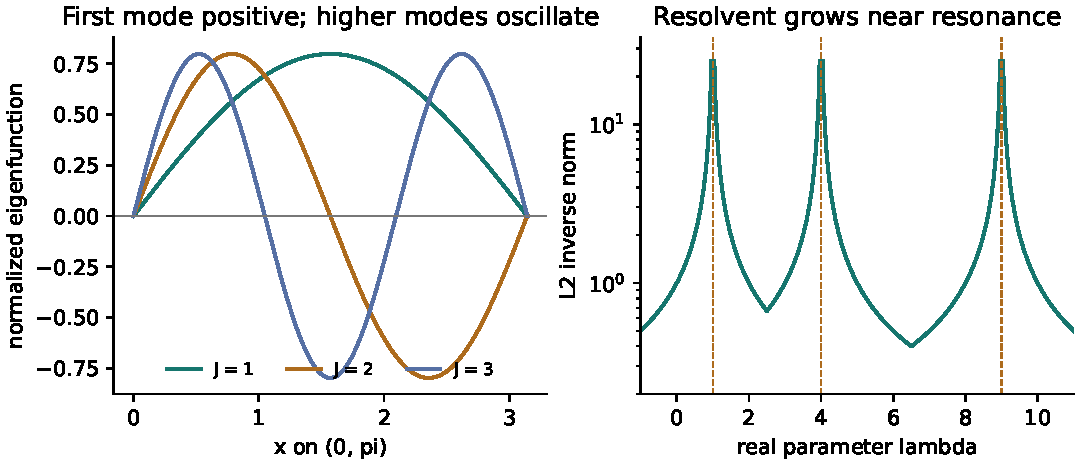
\includegraphics[width=\linewidth]{output/figures/ch06-modes-resonance.pdf}
\end{center}
{\small\textit{Explicit interval model.} On $(0,\pi)$ the Dirichlet
eigenvalues are $j^2$. For real $\lambda$ off the spectrum, the
self-adjoint inverse norm is
$\|(-\partial_{xx}-\lambda)^{-1}\|_{L^2\to L^2}
=1/\min_j|j^2-\lambda|$. The poles mark loss of uniqueness.}
\end{minipage}

\paragraph{Weyl's law: a source remark, not a proved theorem here.}
For the Dirichlet Laplacian on a smooth bounded domain,
\[
 N(\lambda):=\#\{j:\lambda_j\leq\lambda\}
 \sim \frac{\omega_n|U|}{(2\pi)^n}\lambda^{n/2}.
\]
Equivalently,
$\lambda_j\sim4\pi^2(j/(\omega_n|U|))^{2/n}$.
This asymptotic statement appears as a remark in Evans; its proof
requires additional spectral estimates and is not part of the
compactness argument above. Here $\omega_n$ is the volume of the unit ball.

% Expanded proof of Evans 6.5.2, Theorem 3; Schaefer is an external prerequisite.
\Needspace{35mm}
\subsection{A positive eigenfunction without symmetry (Evans \S6.5.2)}
Now write $L=-a^{ij}\partial_{ij}+b^i\partial_i+c$ and assume $c\geq0$.
The matrix $A$ is symmetric, but the full operator need not be self-adjoint.
For weak formulations and adjoints, first rewrite it in divergence form:
the drift in $B$ is $b^i+\partial_j a^{ij}$, rather than $b^i$ itself.

\begin{theorem}\label{thm:6-principal-nonsym}
There is a real eigenvalue $\lambda_1>0$ and an eigenfunction
$\phi>0$ in $U$, $\phi=0$ on $\partial U$.
Its eigenspace is one dimensional. Every complex eigenvalue $\lambda$
satisfies $\operatorname{Re}\lambda\geq\lambda_1$.
\end{theorem}
\Needspace{45mm}
\PDEAnnotation{非对称时换一种结构}{非对称算子通常没有正交特征基，Rayleigh 商也不再直接给出全部谱。主特征值的存在依赖紧逆算子保持非负性，极小实部则由正特征函数的商变换证明。}
\begin{expandedproof}
\paragraph{1. Construct a positive compact inverse.}
The homogeneous zero-Dirichlet problem has only the zero solution:
regularity makes a weak homogeneous solution classical, and comparison
applied to both signs gives zero. Fredholm therefore supplies $T=L^{-1}$.
Fix an integer $m>n/2+2$ and let $X=H^m(U)\cap H^1_0(U)$ with its $H^m$
norm. Boundary regularity makes $T:X\to H^{m+2}(U)\cap H^1_0(U)$ bounded,
so $T:X\to X$ is compact.
The closed convex cone $\mathcal C=\{u\in X:u\geq0\}$ is preserved by $T$.

Fix $0\ne w\in C^\infty_c(U)$, $w\geq0$.
The strong minimum principle and Hopf's lemma imply
$Tw>0$ inside and $\partial_\nu(Tw)<0$ on the boundary.
Since $w$ has compact support, some $\mu>0$ satisfies $\mu Tw\geq w$.

\paragraph{2. A compact fixed-point argument yields an eigenvector.}
We invoke the following \emph{external} form of Schaefer's theorem:
if a continuous compact map $F:\mathcal C\to\mathcal C$ has a bounded
set $\{u:u=tF(u),\ 0\leq t\leq1\}$, then $F$ has a fixed point.
This topological theorem is a prerequisite here, not proved in this chapter.

For $\varepsilon>0$, consider
\[
 u=\eta T(u+\varepsilon w),\qquad u\in\mathcal C.
\]
No solution can have $\eta>\mu$. Indeed positivity gives
$u\geq\varepsilon(\eta/\mu)w$; iterating $u\geq\eta Tu$ gives
$u\geq\varepsilon(\eta/\mu)^kw$ for every $k$, impossible at a point
where $w>0$.
If the solutions for $0\leq\eta\leq2\mu$ were bounded, Schaefer applied
to $F(u)=2\mu T(u+\varepsilon w)$ would give a solution at $\eta=2\mu$,
a contradiction. Hence that solution set is unbounded.
Choose $\varepsilon_j\downarrow0$ and solutions $u_j,\eta_j$ with
$\|u_j\|_X\geq\varepsilon_j^{-1}$ and $0\leq\eta_j\leq2\mu$.
Normalize $v_j=u_j/\|u_j\|_X$. Then
\[
 v_j=\eta_j T\left(v_j+\frac{\varepsilon_jw}{\|u_j\|_X}\right).
\]
Compactness gives a subsequence converging in $X$ to $v$ with
$\|v\|_X=1$, $v=\eta Tv$, and $\eta>0$ (otherwise the right side
would converge to zero). Thus $Lv=\eta v$, $v\geq0$.
Regularity, the strong minimum principle and Hopf give a smooth
$\phi=v>0$, $\partial_\nu\phi<0$, with $\lambda_1=\eta>0$.

\Needspace{45mm}
\PDEAnnotation{归一化保住非零极限}{紧性本身可能只给出零极限。把无界解列除以自身范数后，范数固定为一；扰动项同时趋零，极限才成为真正的非零特征函数。}
\paragraph{3. Exclude eigenvalues to the left of $\lambda_1$.}
For a complex eigenfunction $z$, smoothness and zero boundary values imply
$|z(x)|\leq C d(x)$ near the boundary, with
$d(x)=\operatorname{dist}(x,\partial U)$.
Hopf and compactness of $\partial U$ give $\phi(x)\geq a d(x)$.
For $0<\delta<1$, put $h=\phi^{1-\delta}$ and $v=z/h$.
Then $v$ extends continuously as zero on $\partial U$.

\PDEMarginDiagram{6.M}{商为何在边界趋零}
{由 $|z|\leq Cd$ 与 $\phi\geq ad$，得到 $|z|/\phi^{1-\delta}\leq C'd^\delta\to0$。图示上界取 $\delta=1/2$。}
{ch06-boundary-ratio-margin}

A product calculation gives
\[
 L(hv)=hKv+vLh,\qquad
 K=-A:D^2+(b-2AD\log h)\cdot D,
\]
and the chain rule gives
\[
 \frac{Lh}{h}
 =(1-\delta)\lambda_1+\delta c+
 \delta(1-\delta)\frac{A D\phi\cdot D\phi}{\phi^2}
 \geq(1-\delta)\lambda_1.
\]
Consequently, for $q=|v|^2$,
\[
 Kq=2\operatorname{Re}(\overline v Kv)-2A Dv\cdot D\overline v
 \leq2\left(\operatorname{Re}\lambda-\frac{Lh}{h}\right)q .
\]
If $\operatorname{Re}\lambda<\lambda_1$, choose $\delta$ small so that
the coefficient on the right is strictly negative.
The nonzero continuous function $q$, zero on $\partial U$, has a
positive interior maximum, where $Dq=0$ and $-A:D^2q\geq0$,
a contradiction. This argument is pointwise at that maximum; it does
not assume the drift $D\log h$ is bounded near the boundary.

\paragraph{4. Prove geometric simplicity by sliding positive functions.}
Let $z$ be a real eigenfunction for $\lambda_1$, changing its sign if
necessary so it is positive somewhere.
The estimates $\phi\geq a d$ and $|z|\leq C d$, also valid after adjusting
constants on the interior compact region, show that
\[
 t_*=\sup\{t\geq0:\phi-tz\geq0\text{ in }U\}
\]
is positive and finite. At $t_*$ the residual $r=\phi-t_*z$ is nonnegative
and satisfies $Lr=\lambda_1r\geq0$.
If it were nonzero, the strong minimum principle and Hopf would give
$r\geq a' d$. Since $|z|\leq C d$, a small further increase of $t_*$
would preserve nonnegativity, a contradiction.
Hence $r=0$. Apply this separately to real and imaginary parts for
complex eigenfunctions at the real value $\lambda_1$.
\end{expandedproof}

\Needspace{35mm}
\subsection{The positive adjoint eigenfunction}
\begin{lemma}\label{lem:6-positive-adjoint}
The formal Dirichlet adjoint has a positive eigenfunction $\phi^*$
for the same $\lambda_1$.
\end{lemma}
\begin{expandedproof}
The inverse $T^*$ is positive on $L^2$: for $f,g\geq0$,
$(T^*f,g)=(f,Tg)\geq0$.
Regularity makes its restriction to $X$ compact.
If $f\in\mathcal C$ is nonzero, $v=T^*f\geq0$ is nonzero.
Although the expanded potential $c^*$ of $L^*$ may be negative,
choose $M$ with $c^*+M\geq0$; then
$(L^*+M)v=f+Mv\geq0$.
The strong minimum principle and Hopf applied to $L^*+M$ give
$v>0$ and $\partial_\nu v<0$.
The compact-cone construction in Steps 1--2, with $T^*$ in place of $T$,
therefore gives $\phi^*>0$ and $L^*\phi^*=\lambda^*\phi^*$, $\lambda^*>0$.
Both eigenfunctions have zero trace, so weak adjointness yields
\[
 \lambda_1(\phi,\phi^*)=B[\phi,\phi^*]
 =(\phi,L^*\phi^*)=\lambda^*(\phi,\phi^*).
\]
The inner product is positive, hence $\lambda^*=\lambda_1$.
\end{expandedproof}
\Needspace{45mm}
\PDEAnnotation{伴随的零阶项可能变号}{原算子的 $c\geq0$ 不推出伴随算子的零阶项非负。先由逆算子的对偶关系得到非负性，再加常数使用强最大值原理，才能严谨得到伴随正特征函数。}
If $c$ has arbitrary sign but is bounded, apply the theorem to $L+\kappa$
with $c+\kappa\geq0$. Translating its eigenvalues back preserves the positive
principal eigenfunction, simplicity and the least-real-part property;
the resulting $\lambda_1$ need not be positive.
The word \emph{simple} above describes the eigenspace. In fact there is
also no generalized eigenvector at $\lambda_1$: an equation
$(L-\lambda_1)z=\phi$ contradicts pairing with $\phi^*$, since
$(\phi,\phi^*)>0$.
